In this section, we detail the design and plugin-based architecture of our framework, which is tailored for the 
systematic collection, standardization, and preprocessing of anatomical MRI data. We discuss (1) the framework's 
modular structure, (2) the functions and interrelationships of each module, and the sequence of data handling 
from acquisition to final output. 

\subsection{Overall Framework Design}

Our framework is developed in Python and utilizes a plugin-based architecture to allow flexible 
substitution or addition of modules without the need for extensive modifications to the core codebase. Each module, 
or plugin, is responsible for a specific aspect of the workflow, such as data downloading from target datasets, 
performing MRI preprocessing, Mapping each of the MRI file to the corresponding dictionary entry (dataset, subject, session),
checking validity of NIfTI files, Visualizing all of the MRI data as well as 
integrating demographic and clinical metadata. 
Figure~\ref{fig:SystemArchitecture} provides a conceptual diagram illustrating the key components and their interactions.


\begin{figure}[htbp]\begin{center}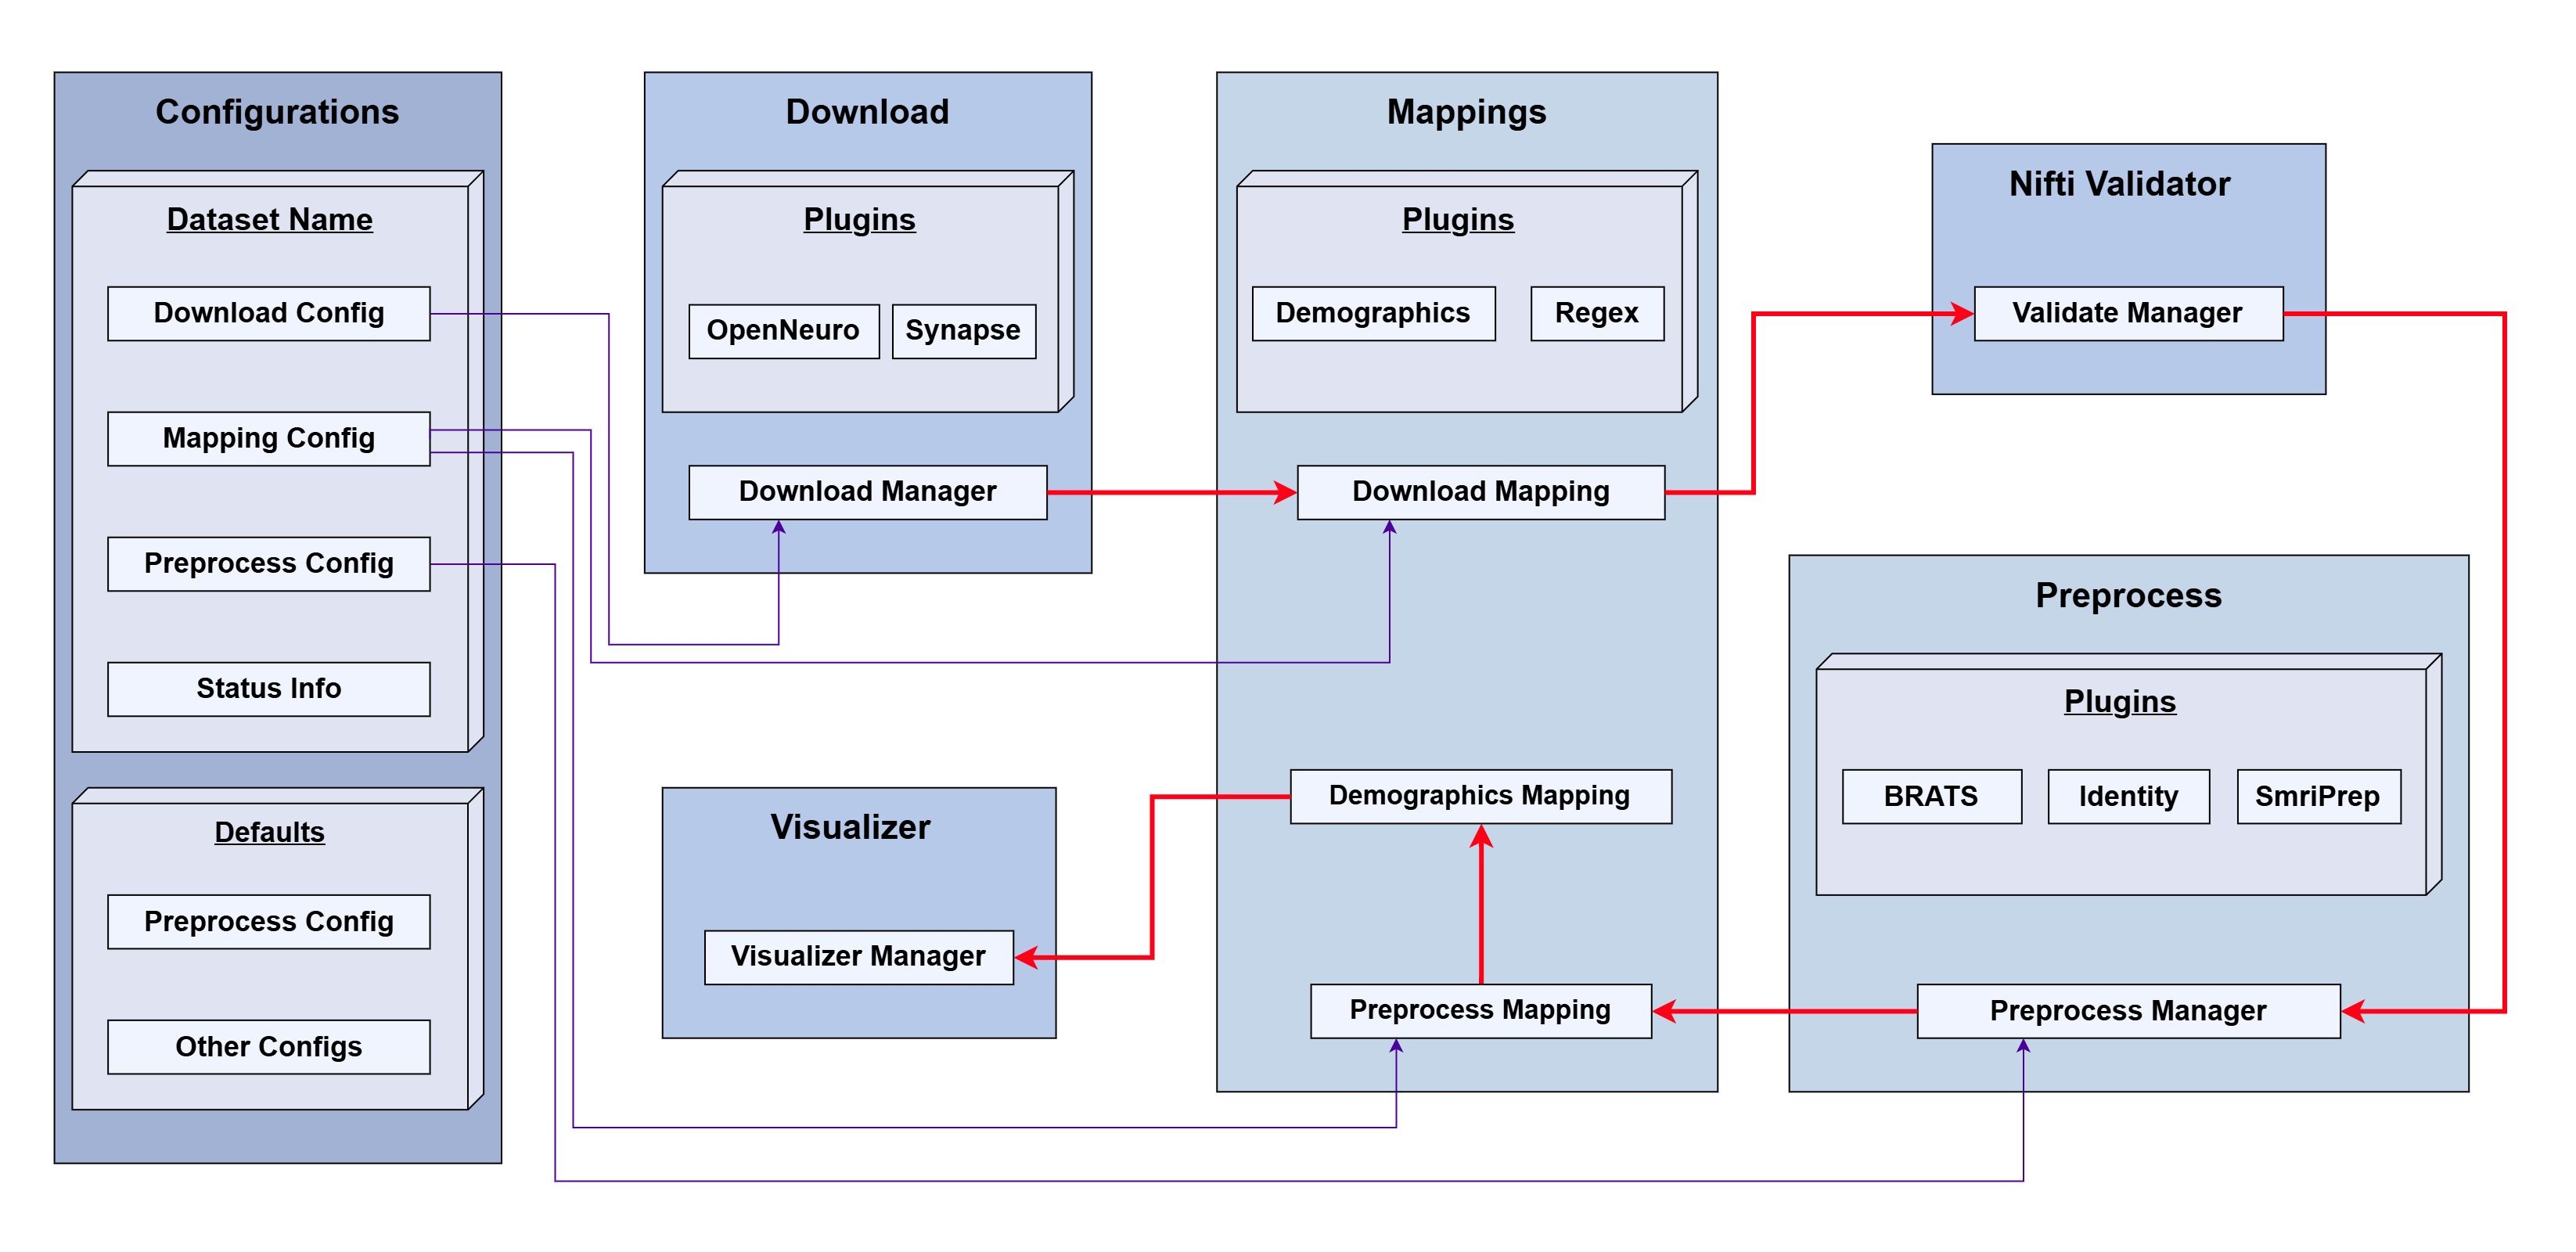
\includegraphics[width=\linewidth]{figures/architecture.png}
    \caption{
        Framework architecture.
    }
    \label{fig:SystemArchitecture}\end{center}
\end{figure}



Key objective of the framework include: 
\begin{description}
    \item[Automation:] Reduce the reliance on manual scripting by automating the processes of dataset downloading, file organization, and data processing.
    \item[Standardization:] Standardize dataset structures by applying regex-based mapping to a uniform data format, and a common preprocessing pipeline across all datasets.
    \item[Extensibility:] Enable the seamless integration of new data sources, additional preprocessing methods, and diverse demographic variables through modular plugins.
    \item[Reproducibility:] Ensure consistent execution and traceability by recording dataset specific download, mapping and processing parameters in JSON configuration files, facilitating accurate replication of the workflow.
\end{description}


\subsection{Plugin-Based Architecture}

This framework incorporates a robust, plugin-based architecture designed to optimize flexibility, scalability, and maintainability in MRI data processing. 
At its core is the Pipeline workflow, which efficiently coordinates the sequential execution of independent modules, ensuring streamlined data flow and 
process synchronization, as illustrated by the red arrows in Figure~\ref{fig:SystemArchitecture}.
The \textbf{Configurations} serves as the central orchestrator of settings which includes default settings across all datasets along with the dataset-specific parameters. 
This approach enables seamless customization, including plugin selection, to accommodate each dataset's requirements when downloading, combining, and preprocessing 
multimodal MRI data from a range of sources with varying data structures.

\textbf{Downloader Plugins}, such as the OpenNeuro downloader (which relies on an \href{https://docs.aws.amazon.com/cli/latest/reference/s3/}{Amazon S3 CLI tool}), 
acquire raw MRI data from multiple repositories. This includes not only OpenNeuro datasets (\cite{markiewicz2021openneuro}) but also other large-scale databases such as the 
Human Connectome Project (HCP) (\cite{van2013wu}). These plugins preserve the source dataset structures, making comparisons more straightforward after downloading.
After acquisition of the target datasets, \textbf{Mapper Plugins} (for instance, the RegexMapper) convert the downloaded MRI data into a standardized JSON record. 
By leveraging user-defined configuration settings, the RegexMapper can accommodate datasets with different file organizations and naming conventions, bringing them into a unified format.
while \textbf{Validator Plugins}, such as the NIfTI Validator, rigorously assess the downloaded MRI data for integrity and compliance, aiding in the early identification of any potential issues 
and ensuring the workflow maintains high standards.

\textbf{Preprocessor Plugins}, such as Brats, Identity, and Smriprep, are employed for specialized tasks including MRI registration, brain extraction, and normalization. 
The Brats preprocessor plugin is particularly preferred for its comprehensive pipeline that mirrors the processes pipeline used in the Brain Tumor Segmentation (BRATS) 
challenge (\cite{menze2014multimodal}), by utilizing \href{https://github.com/BrainLesion/preprocessing}{BrainLes-Preprocessing} tool to perform these preprocessing. 
The Brats pipeline include Co-registration where the moving modalities are co-registered to a central modality (for instance, T1w), followed by atlas registration of the MRI modalities
to the SR24 atlas (\cite{rohlfing2010sri24}), followed by brain extraction, and image intensity normalization. For datasets that have already been brain-extracted and skull-stripped, 
the "Identify" preprocessor is utilized which copies files from the download directory to the preprocess directory, preserving a consistent structure. 
\textbf{Mapper plugins} then updated the datset records by including the processed MRIs, while the \textbf{Demographics Mapper} facilitates seamless integration of demographic 
or clinical data by attaching relevant demographic details to each corresponding dataset record. This modular framework streamlines updates and maintenance 
by allowing plugins to be replaced or customized without affecting the core system, and it empowers researchers to incorporate specialized processes suited to each project. 
As a result, the plugin-based architecture fosters a robust, adaptable MRI data processing workflow that can scale to address diverse research requirements.


\subsubsection{Demographics Information}



A total of \TotalSubjectsIncludedAfterInspectionCount\ subjects were included after inspection 
from a total of \NumDatasets\ datasets. Of these, \TotalSubjectsWithDemographicsInfoCount\ subjects 
have demographic information, while \TotalSubjectsWithoutDemographicsInfoCount\ 
subjects lack any recorded demographic details. The demographic data include age, sex, race, handedness, education level, 
socio-economic status, body mass index, and brain disorders. Table~\ref{DemographicsOverviewTable} provides a comprehensive 
overview of the availability of each demographic field across all of the datasets.



\begin{table}[h!]
    \centering
    \begin{threeparttable}
        \caption{Count of Subjects with Each Demographic Field}
        \label{DemographicsOverviewTable}
        \setlength{\tabcolsep}{45pt}%
        
        \begin{tabular}{@{}ll}
            \toprule
            \textbf{Demographic Field} & \textbf{Number of Subjects} \\
            \midrule
            Age & \TotalSubjectsWithAgeCount\ \\
            Age Group & \TotalSubjectsWithAgeGroupCount\ \\
            Sex (Gender) & \TotalSubjectsWithSexCount\ \\
            Handedness & \TotalSubjectsWithHandednessCount\ \\
            Race & \TotalSubjectsWithRaceCount\ \\
            Education & \TotalSubjectsWithEducationCount\ \\
            Socio-Economic Status & \TotalSubjectsWithSocioEconomicCount\ \\
            Body Mass Index & \TotalSubjectsWithBodyMassIndexCount\ \\
            Brain Disorders & \TotalSubjectsWithDisordersCount\ \\
            No Demographics & \TotalSubjectsWithoutDemographicsInfoCount\ \\
            \bottomrule
        \end{tabular}
        
        \begin{tablenotes}[flushleft]\footnotesize
            \item[${a}$] Basic counts of demographic coverage across the dataset.
        \end{tablenotes}
    \end{threeparttable}
\end{table}


It is evident that \textit{age} (or \textit{age group}) and \textit{sex} are among the most crucial and commonly analyzed demographics. 
According to Table~\ref{DemographicsOverviewTable}, \TotalSubjectsWithAgeCount\ subjects have an explicit \textit{age} value, 
\TotalSubjectsWithAgeGroupCount\ scans include a recorded \textit{age group} label, and \TotalSubjectsWithSexCount\ scans have \textit{sex} information. 
Of these, \TotalSubjectsWithAgeAgeGroupSexCount\ scans possess both age (or age group) and sex information.


\begin{figure}[ht]
    \centering
    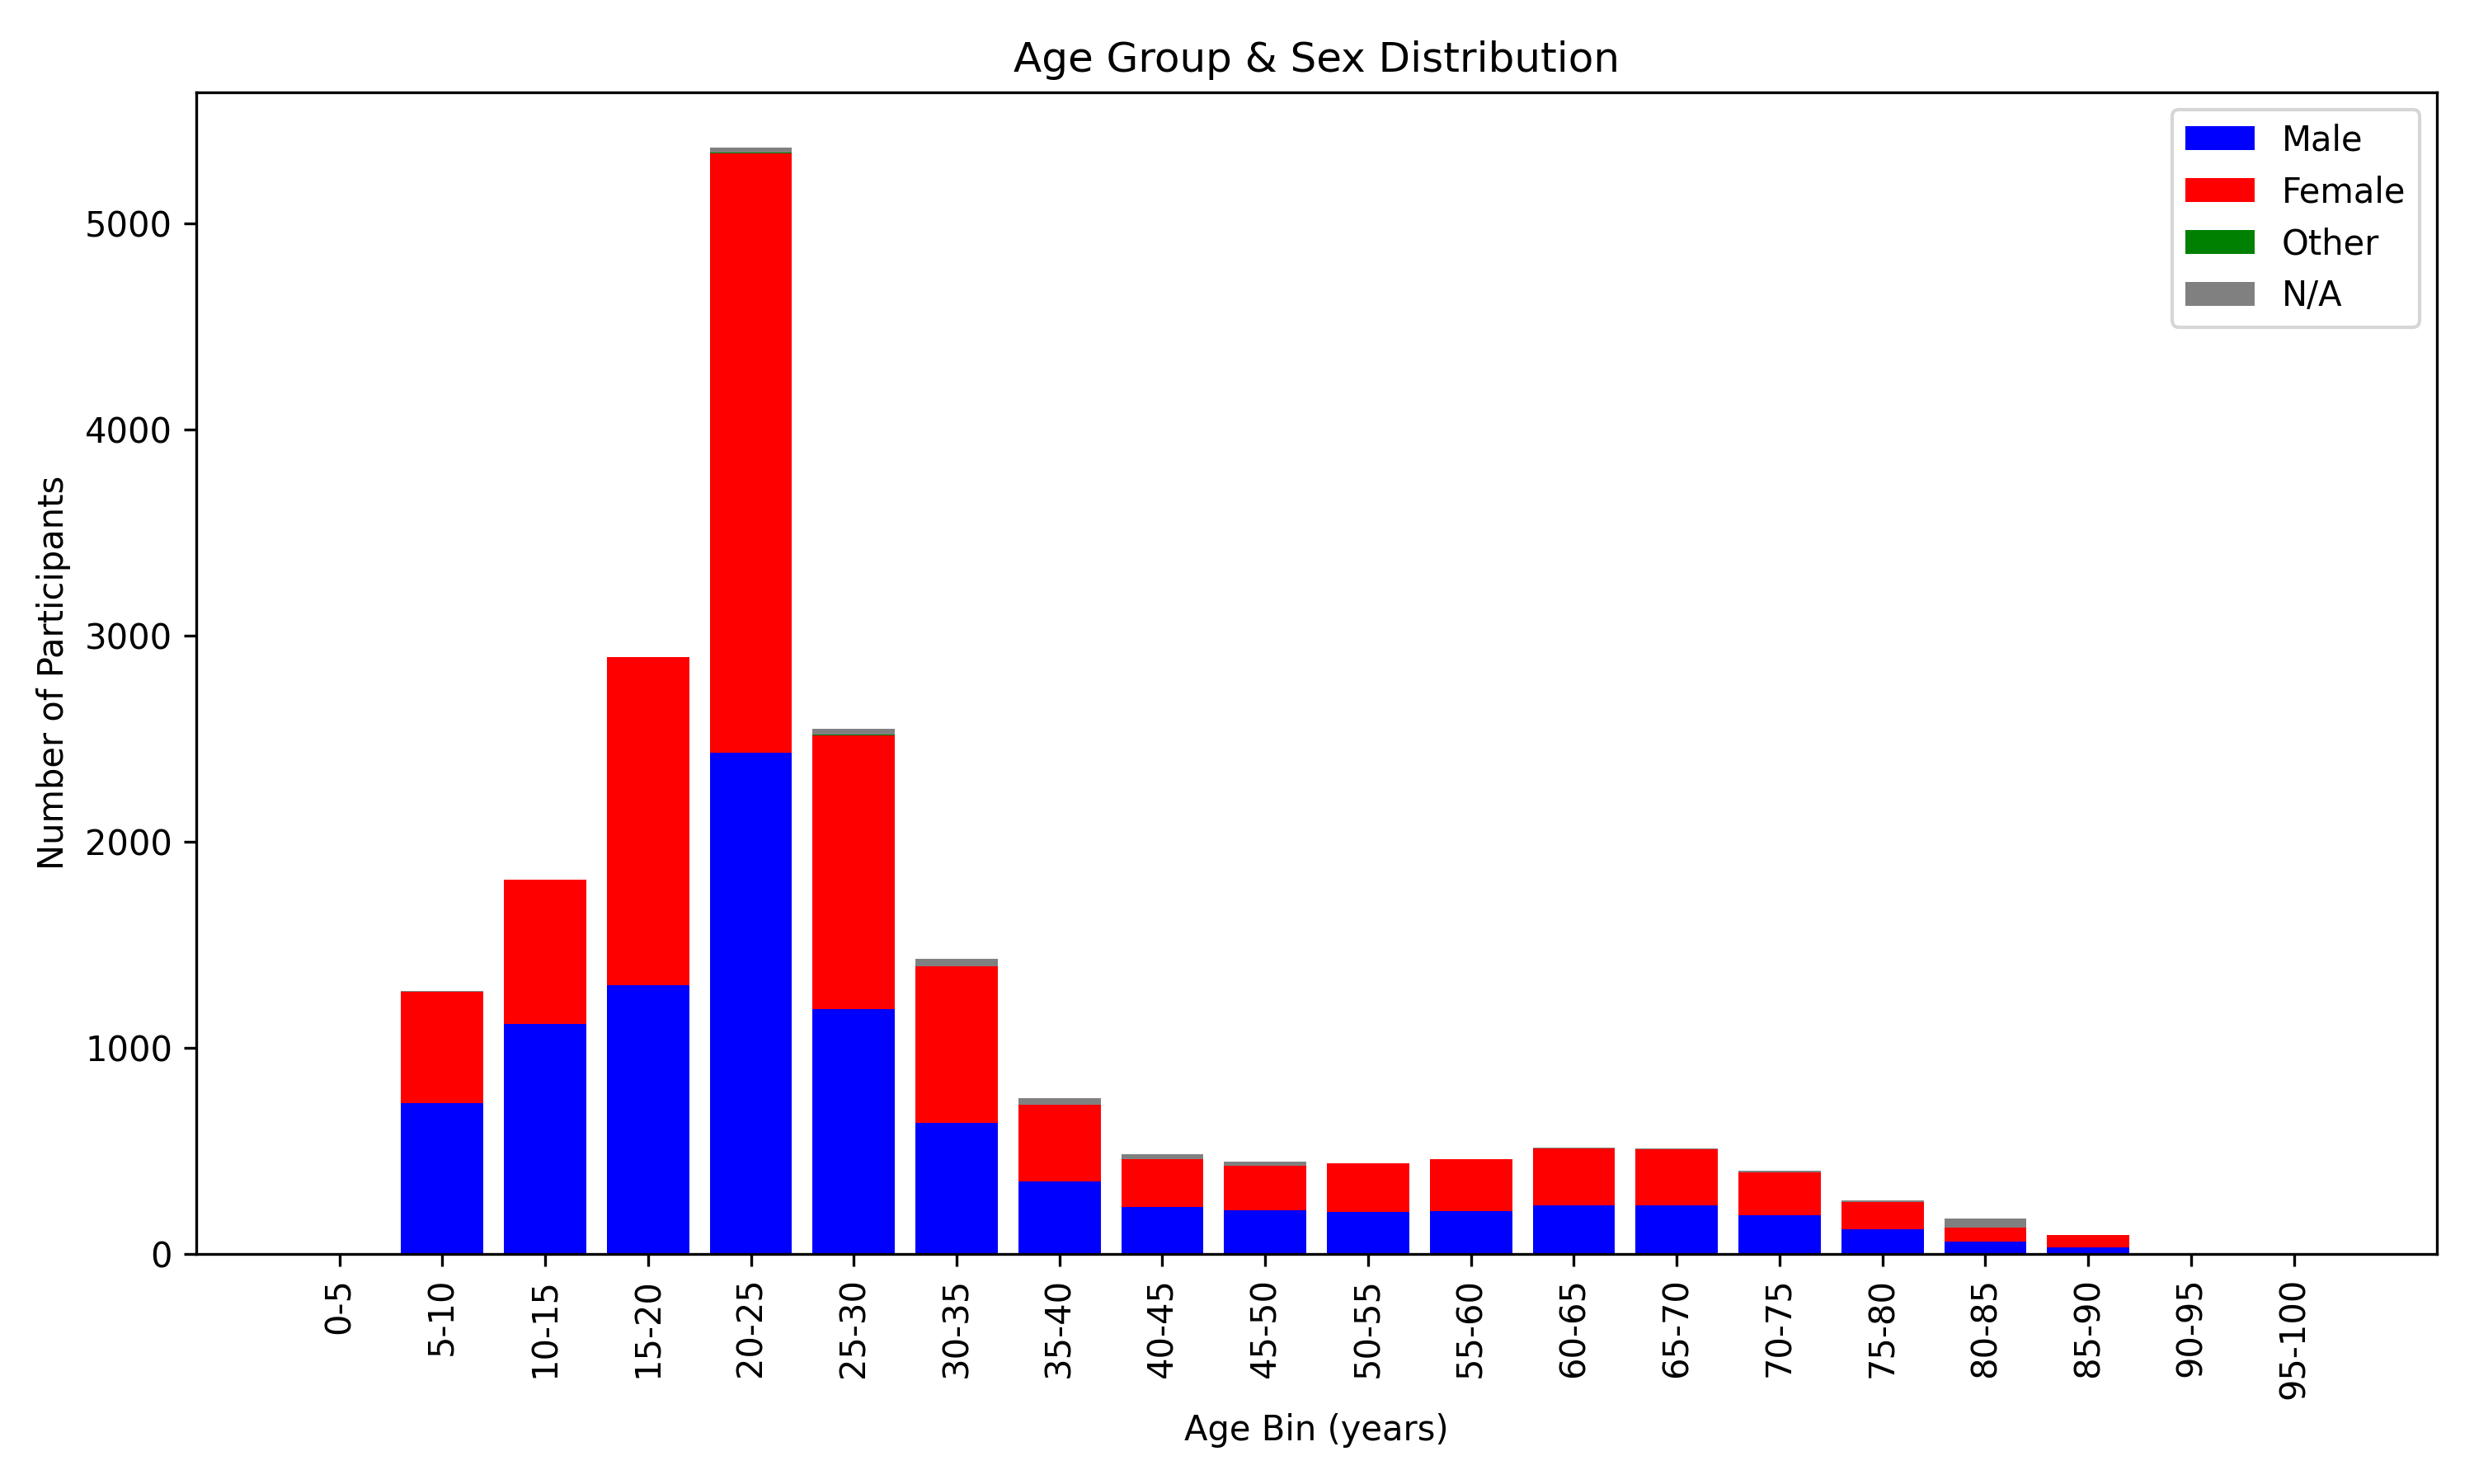
\includegraphics[width=\linewidth]{figures/age_group_sex_histogram} 
    \caption{Histogram of Age (or Age Groups) by Sex. Each bar represents a bin of age or an age group, subdivided by sex categories (male, female, other, n/a).}
    \label{HistogramAgeSexFigure}
\end{figure}


\noindent
Figure~\ref{HistogramAgeSexFigure} presents a histogram illustrating how the dataset's age distribution is subdivided by sex categories. 
Specifically, the histogram organizes \textit{age} (or \textit{age group}) into bins along the horizontal axis, whereas the vertical bars 
representing the participants count, color-coded to indicate the categories: "male", "female", "other", and "n/a". Note: \TotalSubjectsWithSexCountWithoutAgeInfo\ 
subjects who have only \textit{sex} information and lack \textit{age} or \textit{age group} data are omitted from the histogram.


Overall, the \textit{mean} age (excluding entries with only age group data) is \TotalSubjectsMeanAgeValue\ (SD = \TotalSubjectsStandardDevValue{}). 
By categorizing individual ages into bins, as illustrated in Figure~\ref{HistogramAgeSexFigure}, the \textit{median} age group is determined to be \TotalSubjectsMedianAgeGroupValue\ years.
The \textit{sex} distribution among subjects with both age and sex data includes \TotalSubjectsWithMaleSexCount\ males, \TotalSubjectsWithFemaleCount\ females, 
and \TotalSubjectsWithOtherSexCount\ individuals identifying as other genders, totaling \TotalSubjectsWithSexCount\ subjects. 

Beyond age and sex, the dataset includes additional demographic information such as race, handedness, education level, and socio-economic status. 
Table~\ref{additional_demographics} shows the distribution of these variables:


\begin{table}[ht]
    \centering
    \begin{threeparttable}
        \caption{Distribution of Demographic Variables}
        \label{additional_demographics}
        \begin{tabular}{@{}lccc@{}}
            \toprule
            \textbf{Variable} & \textbf{Category/Level} & \textbf{Count (n)} & \textbf{Percentage (\%)} \\
            \midrule
            \textbf{Race}   & White & \TotalSubjectsWithWhiteRaceCount & \TotalSubjectsWithWhiteRacePercentage \\
                            & Black & \TotalSubjectsWithBlackRaceCount & \TotalSubjectsWithBlackRacePercentage \\
                            & Asian & \TotalSubjectsWithAsianRaceCount & \TotalSubjectsWithAsianRacePercentage \\
                            & American Indian/Alaska Native & \TotalSubjectsWithAmericanIndianAlaskanRaceCount & \TotalSubjectsWithAmericanIndianAlaskanRacePercentage \\
                            & Hawaiian/Pacific Islander & \TotalSubjectsWithHawaiianPacificIslanderRaceCount & \TotalSubjectsWithHawaiianPacificIslanderRacePercentage \\
                            & Two or More Races & \TotalSubjectsWithTwoOrMoreRaceCount & \TotalSubjectsWithTwoOrMoreRacePercentage \\
                            & Other & \TotalSubjectsWithOtherRaceCount & \TotalSubjectsWithOtherRacePercentage \\
            \textbf{Handedness} & Right (R) & \TotalSubjectsWithRightHandednessCount & \TotalSubjectsWithRightHandednessPercentage \\
                                & Left (L) & \TotalSubjectsWithLeftHandednessCount & \TotalSubjectsWithLeftHandednessPercentage \\
                                & Ambidextrous (A) & \TotalSubjectsWithAmbidextrousHandednessCount & \TotalSubjectsWithAmbidextrousHandednessPercentage \\
            \textbf{Education} & Low (Primary/HS) & \TotalSubjectsWithLowEducationCount & \TotalSubjectsWithLowEducationPercentage \\
                               & Medium (College) & \TotalSubjectsWithMediumEducationCount & \TotalSubjectsWithMediumEducationPercentage \\
                               & High ($\geq$ Masters) & \TotalSubjectsWithHighEducationCount & \TotalSubjectsWithHighEducationPercentage \\
            \textbf{Socio-Economic Status}  & Low & \TotalSubjectsWithLowEconomicCount & \TotalSubjectsWithLowEconomicPercentage \\
                                            & Medium & \TotalSubjectsWithMediumEconomicCount & \TotalSubjectsWithMediumEconomicPercentage \\
                                            & High & \TotalSubjectsWithHighEconomicCount & \TotalSubjectsWithHighEconomicPercentage \\
            \bottomrule
        \end{tabular}
        \begin{tablenotes}[flushleft]\footnotesize
            \item[${a}$] Frequencies and percentages of race, handedness, education, and socio-economic status.
        \end{tablenotes}
    \end{threeparttable}
\end{table}





\noindent
Table~\ref{additional_demographics} shows that out of the total \TotalSubjectsWithRaceCount\ subjects with race information,
\TotalSubjectsWithWhiteRaceCount\ participants (\TotalSubjectsWithWhiteRacePercentage\%) self-identified 
as White, \TotalSubjectsWithBlackRaceCount\ (\TotalSubjectsWithBlackRacePercentage\%) as Black or African American, \TotalSubjectsWithAsianRaceCount\
(\TotalSubjectsWithAsianRacePercentage\%) as Asian, and so forth. Furthermore, the majority of participants were right-handed 
(\TotalSubjectsWithRightHandednessCount\ subjects, \TotalSubjectsWithRightHandednessPercentage\%), with smaller proportions of left-handed 
(\TotalSubjectsWithLeftHandednessCount\ subjects, \TotalSubjectsWithLeftHandednessPercentage\%) and ambidextrous individuals 
(\TotalSubjectsWithAmbidextrousHandednessCount\, \TotalSubjectsWithAmbidextrousHandednessPercentage\%). 

Educational information of \TotalSubjectsWithEducationCount\ subjects from different dataset is classified into three categories: low, medium, and high. 
Low educational attainment (\TotalSubjectsWithLowEducationCount\ subjects, \TotalSubjectsWithLowEducationPercentage\%) comprises primary and high school education, 
medium (\TotalSubjectsWithMediumEducationCount\ subjects, \TotalSubjectsWithMediumEducationPercentage\%) includes college, diploma, or Associate's Degree, 
and high (\TotalSubjectsWithHighEducationCount\ subjects, \TotalSubjectsWithHighEducationPercentage\%) involves participants with bachelor's, master's, or PhD degrees. 
Similarly, socio-economic status is categorized as low (\TotalSubjectsWithLowEconomicCount\ subjects, \TotalSubjectsWithLowEconomicPercentage\%), 
medium (\TotalSubjectsWithMediumEconomicCount\ subjects, \TotalSubjectsWithMediumEconomicPercentage\%), and high (\TotalSubjectsWithHighEconomicCount\ subjects, 
\TotalSubjectsWithHighEconomicPercentage\%) distributions.




\subsubsection{Mental Disorders and Clinical Conditions}

A total of \TotalSubjectsWithDisordersCount\ participants in the dataset have been diagnosed with one or more disorders, including stroke, 
tumor, epilepsy, ADHD, bipolar disorder, prosopagnosia, and others. Table~\ref{mental_disorders} lists how many subjects were diagnosed 
with each disorder out of the overall \TotalSubjectsIncludedAfterInspectionCount\ individuals. 


\begin{table}[ht]
    \centering
    \begin{threeparttable}
        \caption{Number of Subjects with Mental Disorders (With Condition Only)}
        \label{mental_disorders}
        \begin{tabular}{@{}lc@{}}
            \toprule
            \textbf{Disorder/Condition} & \textbf{Number of Subjects} \\
            \midrule
            Stroke & \SubjectsWithStrokeCount\ \\
            Schizophrenia & \SubjectsWithSchizophreniaCount\ \\
            Depression & \SubjectsWithDepressionCount\ \\
            ADHD & \SubjectsWithADHDCount\ \\
            Bipolar Disorder & \SubjectsWithBIPOLARCount\ \\
            Prosopagnosia & \SubjectsWithProsopagnosiaCount\ \\
            Epilepsy & \SubjectsWithEpilepsyCount\ \\
            Tumor & \SubjectsWithTumorCount\ \\
            Acute Ischemic Stroke & \SubjectsWithAcuteIschemicStrokeCount\ \\
            Focal Cortical Dysplasia & \SubjectsWithFCDCount\ \\
            Hippocampal Sclerosis & \SubjectsWithHSCount\ \\
            DNT & \SubjectsWithDNTCount\ \\
            Gliosis & \SubjectsWithGLCount\ \\
            Aneurysm & \SubjectsWithAneurysmCount\ \\
            \bottomrule
        \end{tabular}
        \begin{tablenotes}[flushleft]\footnotesize
            \item[${a}$] Only participants who tested \texttt{Y} (Yes) for each disorder are counted here.
        \end{tablenotes}
    \end{threeparttable}
\end{table}


\noindent
Table~\ref{mental_disorders} highlights that \SubjectsWithStrokeCount\ participants have been 
diagnosed with stroke, \SubjectsWithEpilepsyCount\ with tumors, and so on. In total, 
\TotalSubjectsWithDisordersCount\ participants present at least one mental disorder. 




\subsubsection{Visual Inspection}



All MRI datasets included in this study underwent a rigorous visual inspection to identify and exclude scans presenting various artifacts, 
including motion artifacts, susceptibility distortions, aliasing (wrap-around) artifacts, and Gibbs (truncation) artifacts. 
Similarly, subjects with poorly defaced MRIs, where portions of the brain were inadvertently removed, were excluded. For transparency and 
traceability, any scan failing visual quality checks is listed in the corresponding dataset's metadata, enabling researchers to audit, 
revisit, or reverse these exclusions if required.


This process has thus far resulted in the removal of \TotalNumSubjectsRemoved\ subjects across \TotalNumDatasetsWithSubjectsRemoved\ datasets 
from the total of \NumDatasets\ included in the repository. Additionally, \NumDatasetsAlreadySkullStripped\ datasets out of the total \NumDatasets\ 
have brain MRIs that were already skull-stripped. However, subjects with poorly skull-stripped MRIs were also excluded. Figure~\ref{dropped_subject} 
illustrates examples of the excluded MRI scans, highlighting the types of artifacts and issues that led to their removal. By making the exclusion 
criteria explicit and open to community re-evaluation, we reduce the risk of perpetuating errors and encourage collaborative quality assurance, 
ultimately enhancing the overall integrity and reproducibility of the dataset.


\begin{figure}[htbp]\begin{center}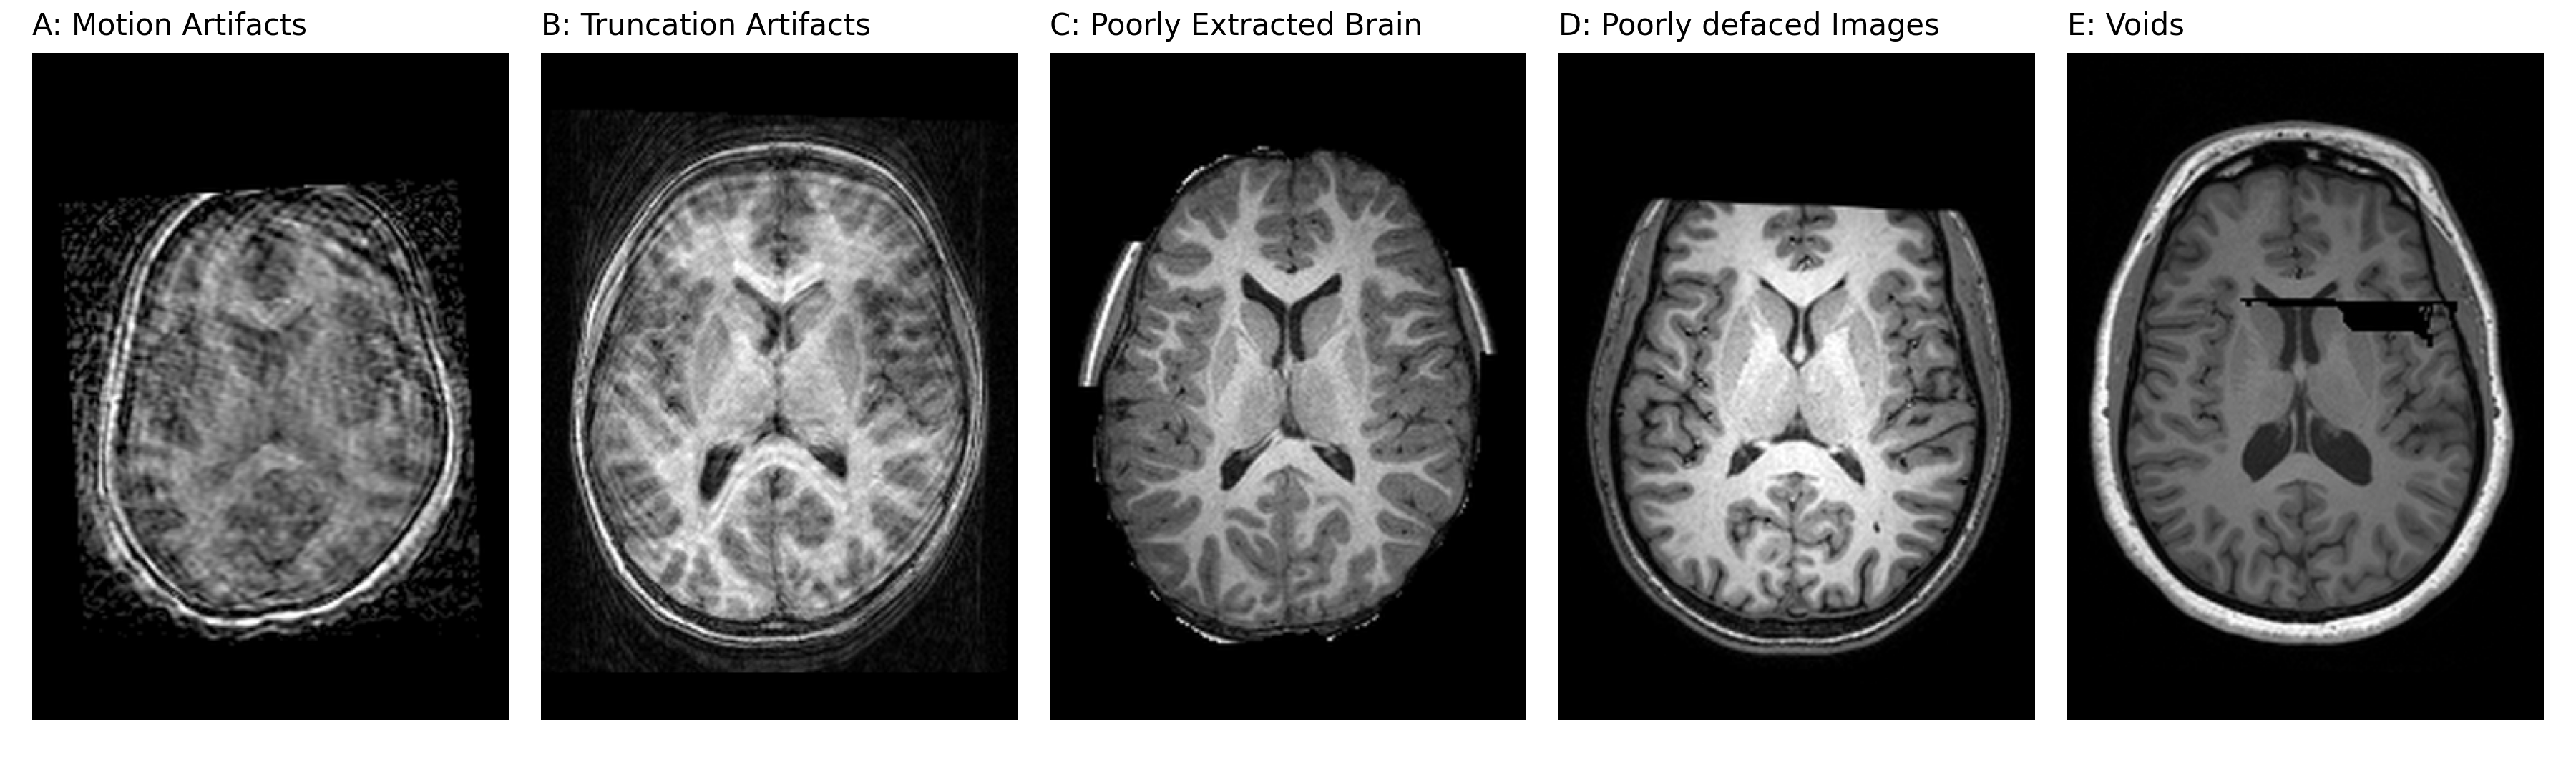
\includegraphics[width=\linewidth]{figures/dropped_subjects.png}
    \caption{
        Examples of MRI scans excluded during visual quality inspection:
        (A) Motion artifacts, 
        (B) Truncation (Gibbs) artifacts, 
        (C) Poorly extracted brain regions, 
        (D) Inadequate defacing with cropped brain regions, 
        and (E) Missing or void pixels.
    }
    \label{dropped_subject}\end{center}
\end{figure}

